%%%% Better Poster latex template example v1.0 (2019/04/04)
%%%% GNU General Public License v3.0
%%%% Rafael Bailo
%%%% https://github.com/rafaelbailo/betterposter-latex-template
%%%% 
%%%% Original design from Mike Morrison
%%%% https://twitter.com/mikemorrison

\documentclass[a0paper,fleqn]{betterposter}

%%%% Uncomment the following commands to customise the format

%% Setting the width of columns
% Left column
\setlength{\leftbarwidth}{0.25\paperwidth}
% Right column
\setlength{\rightbarwidth}{0.25\paperwidth}

%% Setting the column margins
% Horizontal margin
%\setlength{\columnmarginvertical}{0.05\paperheight}
% Vertical margin
%\setlength{\columnmarginhorizontal}{0.05\paperheight}
% Horizontal margin for the main column
%\setlength{\maincolumnmarginvertical}{0.15\paperheight}
% Vertical margin for the main column
%\setlength{\maincolumnmarginhorizontal}{0.15\paperheight}

%% Changing font sizes
% Text font
%\renewcommand{\fontsizestandard}{\fontsize{28}{35} \selectfont}
% Main column font
%\renewcommand{\fontsizemain}{\fontsize{28}{35} \selectfont}
% Title font
\renewcommand{\fontsizetitle}{\fontsize{69} \selectfont}
% Author font
%\renewcommand{\fontsizeauthor}{\fontsize{28}{35} \selectfont}
% Section font
%\renewcommand{\fontsizesection}{\fontsize{28}{35} \selectfont}

%% Changing font sizes for a specific text segment
% Place the text inside brackets:
% {\fontsize{28}{35} \selectfont Your text goes here}

%% Changing colours
% Background of side columns
%\renewcommand{\columnbackgroundcolor}{black}
% Font of side columns
%\renewcommand{\columnfontcolor}{gray}
% Background of main column
%\renewcommand{\maincolumnbackgroundcolor}{empirical}
%\renewcommand{\maincolumnbackgroundcolor}{theory}
%\renewcommand{\maincolumnbackgroundcolor}{methods}
%\renewcommand{\maincolumnbackgroundcolor}{intervention}
% Font of main column
%\renewcommand{\maincolumnfontcolor}{gray}

\begin{document}	
\betterposter{
%%%%%%%% MAIN COLUMN

% Some ideas from Katy
% -> Bus factor analysis
% -> Review criteria in JOSS
% -> What do we learn from reviewing all these pieces of work?
% -> How many papers usbmitted to JOSS fail to be reproducible, sustainable?
% -> Experience on ease of adoption of new tools (GH Actions?)
% -> Casual commentary about some of the data on adoption of these practices
% -> Frequency of sunmissions to JOSS
% -> https://joss.readthedocs.io/en/latest/review_checklist.html
% -> Talk about the dependcy 
% -> Focus on the struggles


%% IDEAS OF MINE
% -> Look at year-old  JOSS submissions and track the following:
% stars, whether or not they have automated testing, whether or not they have some kind of way to intetreact with users
\maincolumn{
%%%% Main space

%Making a \textbf{discoverable record} of software design decisions and \textbf{comprehensive} webhosted docs elevates the sustainability of small software projects and kickstarts their communities
Small open source projects reliant on non-open components may struggle to attract users. Adding support for open alternatives to these components will attract users.
}{
%%%% Bottom space
%% ADD QR CODE to 
%% QR code
\qrcode{img/saltproc-qr.png}{img/smartphoneWhite}{
\textbf{Take a picture} to
\\check out SaltProc
}
% Smartphone icon
% Author: Freepik
% Retrieved from: https://www.flaticon.com/free-icon/smartphone_65680

%% Compact QR code (comment the previous command and uncomment this one to switch)
%\compactqrcode{img/qrcode}{
%\textbf{Take a picture} to
%\\download the full paper
%}

}

}{
%%%%%%%% LEFT COLUMN

\title{Building sustainability and community in a small project: lessons from working on\\ SaltProc}
\author{Oleksandr R. Yardas}
\author{Dr. Madicken Munk}
\institution{University of Illinois Urbana Champaign}


%\section{SaltProc}
%Sustainable software is maintainable, extendable, and has an active user community, but there is no one agreed-upon definition for "sustainability" in the existing literature \cite{venters_sustainable_2023}.
\vspace{-2cm}
\section{Introduction}
SaltProc is a Python package for simulating nuclear fuel reprocessing created as part of a dissertation project. It was originally built around an export-controlled software project. I took over as maintainer after the original author was unable to continue working on the project. The project had essentially no users, but I did not want to see SaltProc die so came up with a plan to make the project easier to use.

% Maybe talk about PyNE here
% 3. PyNE: a product of the time it was made in 
\vspace{-1cm}
\section{What we did}
\vspace{-2cm}
\begin{itemize}
    \item Set up GitHub Discussions to record design decisions and as a platform to interact with users
    \item Added support for an open-source alternative to Serpent2
    \item Overhauled the web hosted docpages with a guide on how to use the package
    \item Used automation tooling to perform rote tasks (releases, updating and deploying docpages, testing)
    \item Replaced a difficult-to-install dependency with friendlier alternatives
\end{itemize}

% Challeneges that still exists:
% 1. We still have no other contributers. In these niche packages, is it inevitable that these packages will decay away? How do we get other contributers? What have other deveoplers done?
% 2. Things I wish I knew going into this? What problems they have?
\vspace{-1cm}
\section{Conclusion}
After implementing the open source feature and creating the discussions page, SaltProc began to get more stars and we saw interaction from users on the discussion page.

\vspace{-1cm}
\section{Open issues}
SaltProc only has one recent contributor. In niche packages like SaltProc, how we get good users who become contributors?
%% This fills the space between the content and the logo
\vfill

%% Institution logo
%\includegraphics[width=\textwidth]{img/logo}\\

}{
%%%%%%%% RIGHT COLUMN
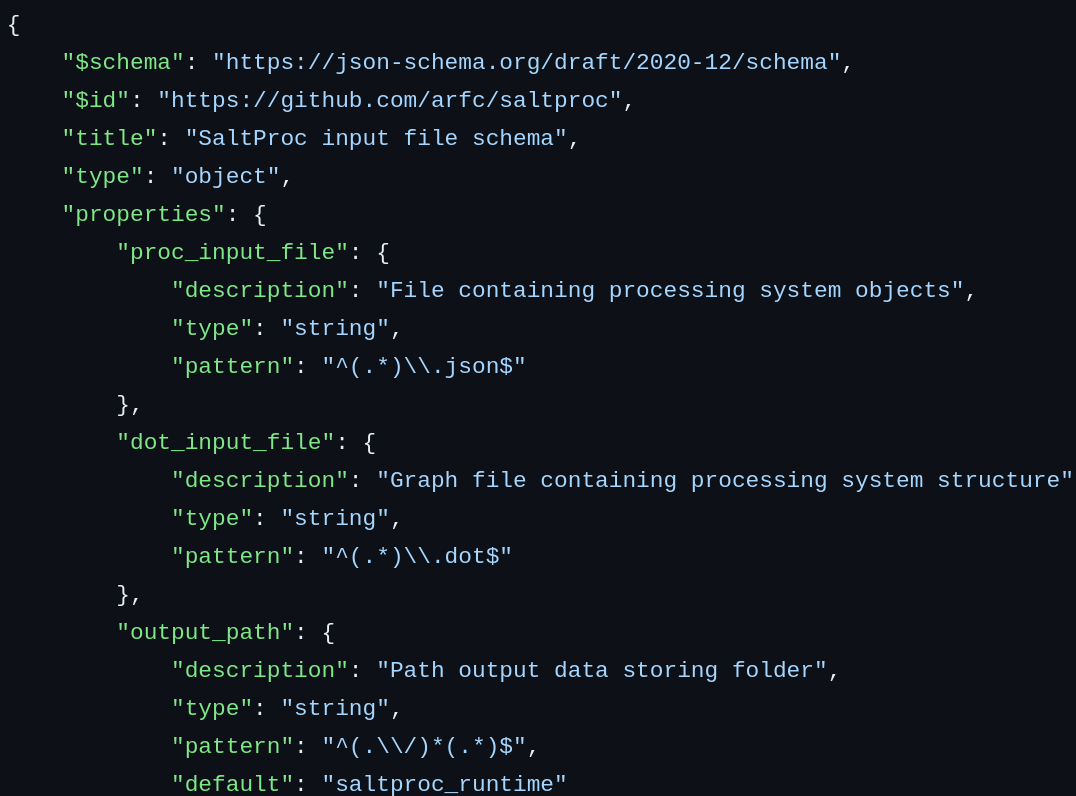
\includegraphics[width=\textwidth]{img/json-schema.png}
\vspace{3cm}
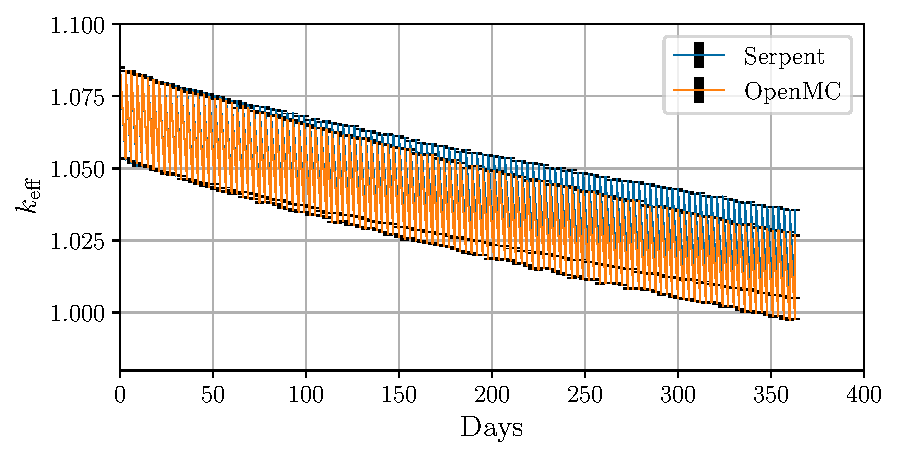
\includegraphics[width=\textwidth]{img/keff.pdf}
\vspace{3cm}
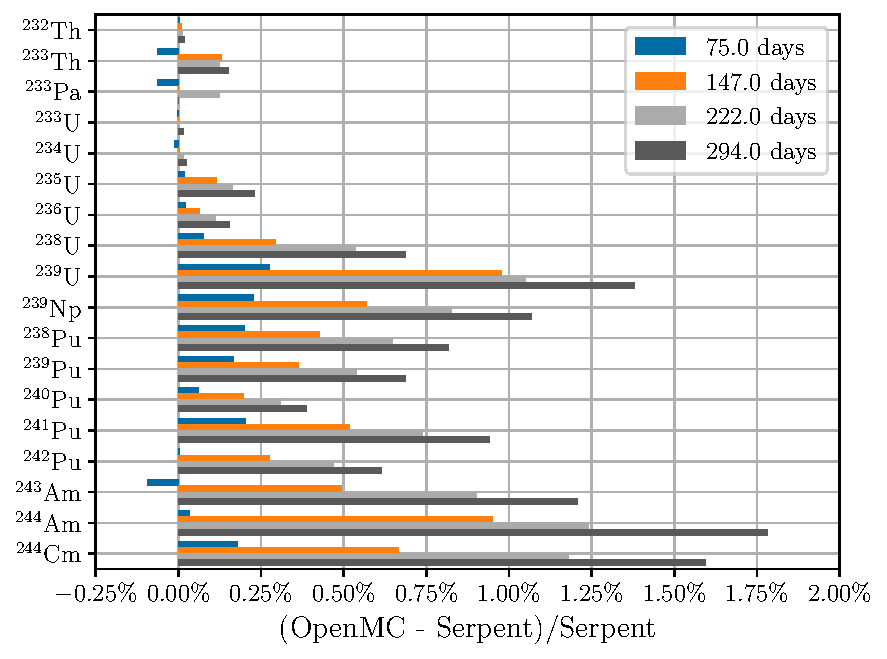
\includegraphics[width=\textwidth]{img/actinides.pdf}
\vspace{3cm}
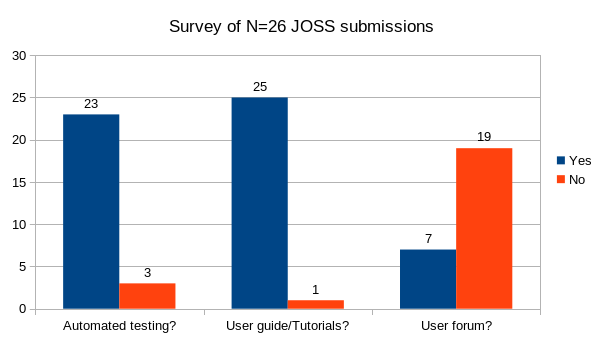
\includegraphics[width=\textwidth]{img/joss-survey.png}
}
\end{document}

